\subsection{Máquina de estados principal}
\label{statemachine}

\begin{figure}[H]
	\centering
	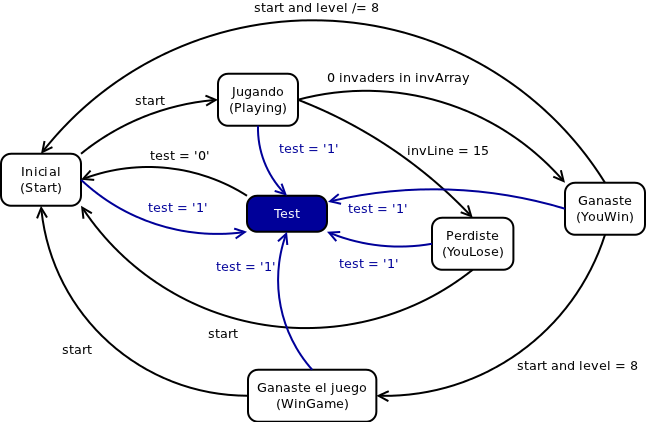
\includegraphics[width=0.6\textwidth]{statemachine.png}
	\caption{Diagrama de estados }\label{fig:statemachine}
\end{figure}

El control del flujo del juego y el funcionamiento de los distintos bloques se lleva a cabo con una máquina de estados. Algunas señales, cuya lógica de activación es más compleja, se activan a partir de las señales de estado en un proceso independiente, que se explicará a continuación. La máquina de estados posee los siguientes estados:

\begin{itemize}
	\item {\bfseries Test}: estado de prueba. Se llega a él desde cualquier estado tras activarse la señal ``test'' y cuando la máquina está en este estado se reinician todos los valores de la partida y se muestra en la pantalla un patrón de tablero de ajedrez.
	\item {\bfseries Inicial (Start)}: en este estado la máquina está esperando que el jugador inicie la partida. Los bloques de ambos jugadores se reincian (excepto las puntuaciones) y desactivan, y el bloque de los invasores se reinicia y permanece parado. Al recibir una señal de inicio ( ``p1StartPulse'') del jugador 1, se pasa al estado ``jugando (playing)''.	
	\item {\bfseries Jugando (Playing)}: este estado corresponde al juego propiamente dicho. En él se inicia el movimiento de los invasores y se habilitan los controles de los jugadores. Desde este estado se pasará a ``ganaste (YouWin)'' si se han eliminado todos los invasores y el vector ``invArray'' sólo contiene `0's, o a ``perdiste (YouLose)'' si los invasores consiguen llegar al final de la pantalla, es decir, si invLine = 15.
	\item {\bfseries Perdiste (YouLose)}: este estado muestra la pantalla de juego perdido. Se permanece en este estado mientras no se reciba una señal de inicio ( ``pxStartPulse'') de cualquiera de los dos jugadores (que lleva la máquina al estado inicial), y en él los invasores y los jugadores permanecen reiniciados y deshabilitados.
	\item {\bfseries Ganaste (YouWin)}: este estado se muestra la pantalla de juego ganado. Se permanece en este estado mientras no se reciba una señal de inicio ( ``pxStartPulse'') de cualquiera de los dos jugadores (que lleva la máquina al estado inicial siempre y cuando no se halla superado el último nivel), y en él los invasores y los jugadores permanecen reiniciados y deshabilitados. Al llegar a este estado se habilita una señal que hace que el contador de nivel se incremente una unidad, haciendo que al volver al estado inicial los invasores que aparezcan sean de una dificultad superior.
	\item {\bfseries Ganaste el Juego (WinGame)}: se llega a este estado tras haber finalizado el último nivel, y en él se muestra la pantalla de juego completado. Este estado reinicia tanto los invasores como los jugadores, y se queda a la espera de una señal de inicio ( ``pxStartPulse'') de cualquiera de los dos jugadores para iniciar una nueva partida.
\end{itemize}

Además de las señales que se controlan de forma combinacional dentro de la máquina de estados, se han añadido algunas señales dependientes del estado o de la transición, cuya lógica de activación es ligeramente más compleja, en procesos independientes. 
Más concretamente, se ha añadido un biestable que contiene la señal de activación del jugador 2, que se acciona cuando nos encontramos en la pantalla de inicio de nivel (``Start'') y recibimos una señal de inicio del jugador 2 (``p2StartPulse), y se reinicia al perder la partida o ganar el juego (una vez el jugador 2 se une a la partida, permanece habilitado hasta que la partida acaba). También se ha añadido un proceso que reinicia las puntuaciones y el nivel cuando se produce una transición desde un estado que no sea ``Ganaste (YouWin)'' hasta el estado ``Inicial (Start)''.